\subsection{Logiciel utilisé}
\subsubsection{Snap!}
\url{http://snap.berkeley.edu/SnapManual.pdf}
Cet partie va donner un aperçu de l'application réutilisée dans ce travail, à savoir Snap!. Comme dit précédemment, cette application est réalisée en JavaScript. La présentation de Snap! va se diviser en plusieurs partie. La première expliquera les différents types de blocs et comment ils sont implémentés. L'exécution d'un programme est l'étape suivante. Enfin, il sera présenté comment l'application affiche les différents éléments la constituant.

\paragraph{Blocs}
Il existe plusieurs type de blocs qui constitue un programme Snap!. Sur l'exemple de programme \ref{fig:software_used_script}, les différents types blocs disponible sont présentés.
\begin{figure}
  \begin{center}
    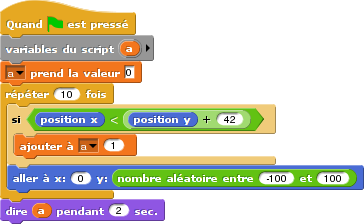
\includegraphics[width=0.5\textwidth]{content/4-theory/2-related_work/images/script}
    \caption{Exemple de programme Snap!}
    \label{fig:software_used_script}
  \end{center}
\end{figure}

\subparagraph{Commande}
Le type principal de bloc est \texttt{commande}. Ces blocs peuvent être compris comme étant des procédures. En effet, les blocs exécutes une ou plusieurs opérations sur le système en fonction des paramètres passés. Ces différents blocs doivent se baser soit sur une implémentation JavaScript pour les commandes élémentaires, soit être une composition de commandes pour fournir une commande plus complexe et/ou abstraite.

Dans l'exemple \ref{fig:software_used_script}, ce sont tout les blocs qui on la forme d'une pièce de puzzle. On peut voir que l'on a une succession de commandes qui crée un script. Les commandes ont plusieurs couleurs suivant la catégorie à laquelle elles appartiennent : mouvement, apparence, contrôles, variable, etc\ldots

\subparagraph{Reporter}
Les reporters sont des fonctions. En effet, ils retournent une valeur. Ils sont toujours utilisés en temps que paramètres d'un autre bloc. La plupart des reporter sont des accesseurs à des variables ou à des états du système (position souris, heure, etc\ldots). 

Les reporters sont les blocs de forme arrondie. L'exemple \ref{fig:software_used_script} montre différente utilisation de reporters : somme, valeur aléatoire, position \ldots Tout comme pour les commandes, les reporters peuvent être de différentes couleurs suivant leur catégorie.

\subparagraph{Prédicat}
Les prédicats sont des reporters qui retournent une valeur booléenne. Ils sont donc utilisés en conjonction avec des commandes demandant une condition.

Les prédicats sont les blocs de forme hexagonale.

\subparagraph{Chapeau}
Les chapeaux sont des commandes spéciales car ils sont le point d'entrée obligatoire d'un script. Ils permettent de démarrer l'exécution d'un script quand un événement se produit.

L'événement qui lancera le script \ref{fig:software_used_script} est donc le démarrage du programme. Celui-ci est symbolisé par un bouton avec drapeau vert.

\paragraph{Programme}
Snap! est plus qu'une interface graphique permettant de construire un programme. L'analyse du fonctionnement interne est l'objet de cette section.

Un programme est constitué de plusieurs processus. Chaque processus sera exécuté en parallèle grâce à un ordonnanceur.

% /*
%     A Process is what brings a stack of blocks to life. The process
%     keeps track of which block to run next, evaluates block arguments,
%     handles control structures, and so forth.
% 
%     The ThreadManager is the (passive) scheduler, telling each process
%     when to run by calling its runStep() method. The runStep() method
%     will execute some number of blocks, then voluntarily yield control
%     so that the ThreadManager can run another process.
% 
%     The Scratch etiquette is that a process should yield control at the
%     end of every loop iteration, and while it is running a timed command
%     (e.g. "wait 5 secs") or a synchronous command (e.g. "broadcast xxx
%     and wait"). Since Snap also has lambda and custom blocks Snap adds
%     yields at the beginning of each non-atomic custom command block
%     execution, and - to let users escape infinite loops and recursion -
%     whenever the process runs into a timeout.
% 
%     a Process runs for a receiver, i.e. a sprite or the stage or any
%     blocks-scriptable object that we'll introduce.
% 
%     structure:
% 
%     topBlock            the stack's first block, of which all others
%                         are children
%     receiver            object (sprite) to which the process applies,
%                         cached from the top block
%     context                the Context describing the current state
%                         of this process
%     homeContext            stores information relevant to the whole process,
%                         i.e. its receiver, result etc.
%     isPaused            boolean indicating whether to pause
%     readyToYield        boolean indicating whether to yield control to
%                         another process
%     readyToTerminate    boolean indicating whether the stop method has
%                         been called
%     isDead              boolean indicating a terminated clone process
%     timeout                msecs after which to force yield
%     lastYield            msecs when the process last yielded
%     errorFlag            boolean indicating whether an error was encountered
%     prompter            active instance of StagePrompterMorph
%     httpRequest         active instance of an HttpRequest or null
%     pauseOffset         msecs between the start of an interpolated operation
%                         and when the process was paused
% */

Un processus \texttt{Process} représente l'exécution d'un script, une pile de blocs. Il assure le suivit de l'exécution du script : prochain bloc à exécuter, objet sur lequel il s'applique (lutin, stage), contexte décrivant l'état courant \ldots

L'ordonnanceur \texttt{ThreadManager} appelle successivement la fonction \texttt{runStep()} (\ref{lst-runstep}) sur chaque processus. Cette fonction exécute un certain nombre de blocs via \texttt{this.evaluateContext()} de manière atomique. Elle rend la main volontairement à l'ordonnanceur quand elle a fini. Comme il est possible d'écrire soi-même des blocs, \texttt{runStep()} rend aussi la main si trop de temps s'est écoulé depuis le début de l'exécution de cette étape. La convention est que les processus rendent la main à la fin de chaque itération de boucle ou quand une opération relative au temps (attendre xxx secondes) ou synchrone (envoyer à tous xxx et attendre la réponse) est exécutée.

\begin{lstlisting}[caption={Fonction \texttt{runStep()} de \texttt{Process}},label=lst-runstep,language=JavaScript]
Process.prototype.runStep = function () {
/*
    a step is an an uninterruptable 'atom', it can consist
    of several contexts, even of several blocks
*/
    // allow pausing in between atomic steps:
    if (this.isPaused) {
        return this.pauseStep();
    }
    this.readyToYield = false;
    while (!this.readyToYield
            && this.context
            && (this.isAtomic ? (Date.now() - this.lastYield < this.timeout) : true) ) {
        // also allow pausing inside atomic steps - for PAUSE block primitive:
        if (this.isPaused) {
            return this.pauseStep();
        }
        this.evaluateContext();
    }
    this.lastYield = Date.now();

    // make sure to redraw atomic things
    if (this.isAtomic &&
            this.homeContext.receiver &&
            this.homeContext.receiver.endWarp) {
        this.homeContext.receiver.endWarp();
        this.homeContext.receiver.startWarp();
    }

    if (this.readyToTerminate) {
        while (this.context) {
            this.popContext();
        }
        // pen optimization
        if (this.homeContext.receiver &&
                this.homeContext.receiver.endWarp) {
            this.homeContext.receiver.endWarp();
        }
    }
};
\end{lstlisting}



% /*
%     A Context describes the state of a Process.
% 
%     Each Process has a pointer to a Context containing its
%     state. Whenever the Process yields control, its Context
%     tells it exactly where it left off.
% 
%     structure:
% 
%     parentContext    the Context to return to when this one has
%                     been evaluated.
%     outerContext    the Context holding my lexical scope
%     expression        SyntaxElementMorph, an array of blocks to evaluate,
%                     null or a String denoting a selector, e.g. 'doYield'
%     receiver        the object to which the expression applies, if any
%     variables        the current VariableFrame, if any
%     upvars          the current UpvarReference, if any (default: null)
%     inputs            an array of input values computed so far
%                     (if expression is a    BlockMorph)
%     pc                the index of the next block to evaluate
%                     (if expression is an array)
%     startTime        time when the context was first evaluated
%     startValue        initial value for interpolated operations
%     activeAudio     audio buffer for interpolated operations, don't persist
%     activeNote      audio oscillator for interpolated ops, don't persist
%     isLambda        marker for return ops
%     isImplicitLambda    marker for return ops
%     isCustomBlock   marker for return ops
%     emptySlots        caches the number of empty slots for reification
% */

\paragraph{GUI}
Un autre élément intéressant à analyser chez Snap! est sa façon d'afficher quelque chose dans la balise html \texttt{canvas}. Toutes les fonctionnalités de base nécessaire à afficher tout éléments graphiques (text rendering, blinking cursors, entry fields, menus, buttons, sliders, windows and dialog boxes \ldots) de Snap! découle de l'implémentation que l'on retrouve dans \texttt{morphic.js}.

\texttt{morphic.js} fournit les abstractions nécessaires à redessiner des parties de l'interface et pour interagir avec l'utilisateur. Le canvas utilisé possède un \texttt{world}. Ce \texttt{world} est la racine de l'arbre composé de \texttt{morph} et leur sous-\texttt{morph}. Chaque \texttt{morph} peut être déplacé, redimensionné via le code ou les manipulations de l'utilisateur.

L'idée principale de \texttt{morphic.js} est de continuellement parcourir tout les éléments du \texttt{world} pour redessiner ceux qui ont été modifié. Le \texttt{world} permet à l'ordonnanceur d'exécuter une étape entre chaque itération. L'exemple \ref{lst-doonecycle} que le monde est rafraîchit toutes les 50 millisecondes.

\begin{lstlisting}[caption={Exemple d'utilisation de \texttt{morphic.js}},label=lst-doonecycle,language=HTML5,alsolanguage=JavaScript]
<!DOCTYPE html>
<html>
    <head>
        <title>Morphic!</title>
        <script type="text/javascript" src="morphic.js"></script>
        <script type="text/javascript">
            var world;

            window.onload = function () {
                world = new WorldMorph(
                    document.getElementById('world'));
                setInterval(loop, 50);
            };

            function loop() {
                world.doOneCycle();
            }
        </script>
    </head>
    <body>
        <canvas id="world" tabindex="1" width="800" height="600" />
    </body>
</html>
\end{lstlisting}

La fonction \texttt{drawNew()} sert dessiner un \texttt{morph}. L'exemple \ref{lst-drawnew} montre que cette fonction dessine son objet sur une image stockée dans l'objet. Cette image provient d'un canvas virtuel généré grâce à l'image du \texttt{morph} parent.

\begin{lstlisting}[caption={Modèle pour la fonction \texttt{drawNew()}},label=lst-drawnew,language=JavaScript]
MyMorph.prototype.drawNew = function() {
    var context;
    this.image = newCanvas(this.extent());
    context = this.image.getContext('2d');
    // use context to paint stuff here
};
\end{lstlisting}

\subsubsection{Rails}
Rails est une plat-forme de développement d'application web basé sur le langage de programmation Ruby. Cette partie présente Rails au travers de sa philosophie, de son architecture et de ses environnements de tests.

\paragraph{Philosophie}
Rails fait l'assomption qu'il existe une meilleur façon d'aborder la création d'application web. Si le programmeur respect ce "Rails way", il améliorera sa productivité et écrira moins de code. D'après Rails, si il persiste à utiliser ses anciennes habitudes, le développeur s'amusera beaucoup moins en développant son application.

Pour atteindre cet objectif, Rails utilise deux principes majeurs :
\begin{description}
  \item[Convention plutôt que configuration] (CoC) Pour permettre au programmeur d'écrire moins de code, Rails permet de n'écrire que ce qui ne correspond pas aux conventions. Rails utilise la méta-programmation pour fournir les conventions à tous les objets;
  \item[Ne vous répétez  pas] (DRY) L'architecture que propose Rails permet de mettre l'information à un endroit unique et bien déterminé. Ceci permet d'avoir un code plus court, plus maintenable, plus extensible et avec moins de bugs.
\end{description}

\paragraph{architecture}
Rails se base sur une architecture Modèle-Vue-Contrôleur.
\subparagraph{Modèle} 
Un modèle est typiquement une classe qui représente une table de la base de données. Une classe du modèle fournit aussi toutes les méthode nécessaire à représenter et modifier l'objet dans le domaine d'application.

La correspondance entre un objet Ruby et la base de données est réalisée grâce à Active Record. Ce module de Rails permet de faire des appels sur des objets Ruby alors que dans d'autres framework, il faudrait utiliser des requêtes SQL.
  
\subparagraph{Contrôleur} 
Le contrôleur permet d'accéder à une ressource. Une ressource est un modèle ou tout autre objet plus indirect (enregistrement/login, page d'accueil\ldots).  

Il détermine quelle vue doit s'afficher et avec quel paramètre. Le contrôleur a donc la tache de vérifier la sécurité et l'intégrité des données fournies par l'utilisateur. Ensuite, il peut interroger différents modèles et fournir les réponses à la vue adéquate. 

Rails encourage d'avoir des ressources REST. C'est a dire, d'avoir des ressources avec une représentations unique et des actions identiques (create, new, edit, update, destroy, show, index). Les actions disponibles sur un contrôleur sont déterminées via le fichier de configuration des routes.

\subparagraph{Vue} 
Les vues sont ce que les utilisateurs reçoivent et voient. Ce sont typiquement des pages html mais aussi des pdf, objets json, fichiers, etc\ldots 

La philosophie de Rails est d'utiliser des gems pour simplifier l'écriture. Pour les vues, nous avons notamment:
\begin{description}
  \item[Haml] un langage fournissant une syntaxe raccourcie du html. Il se base sur l'indentation plutôt que sur une syntaxe XML. Haml permet donc de respecter le principe DRY et d'amélioré la lisibilité par code plus court et bien indenté;
  \item[JQuery] Cette bibliothèque javaScript bien connue permet de modifier le document courant facilement, de géré des événements, de crée des annimation, etc\ldots
  \item[CoffeeScript] Est un langage qui se compile en JavaScript. Il permet d'avoir une syntaxe plus claire et plus courte, il permet d'ajouter des sucre syntaxique par rapport à JavaScript;
  \item[Bootstrap] un framework CSS qui permet de découpler le fond de la forme de l'affichage d'une page html. Ce framework donne un design responsive pour tout type d'écran au page qui l'utilise. Il fournit aussi de nombreux composants utiles (boutons, alertes, barre de progression, message d'aide \ldots).
\end{description}

\paragraph{gem}
Ruby fourni de base une manière de partager des extenstions pour des programmes ruby via les gems. Rails est un gem et dépend de nombreux autres notament Active Record présenté plus haut.

La communauté de Rails à écrit de nombreux gems permettant de rajouter facilement des fonctionnalités à une application. Des gems intéressantes seraint les suivantes :
\begin{description}
  \item[Paperclip] permet de facilement récupérer et stoquer des fichiers. Paperclip permet donc d'intégrer la gestion de fichier tiers de manière propre dans une classe du modèle. Il fourni notament divers drivers pour stoquer ceux-ci aussi bien en local que sur le cloud d'amazon ou de dropbox.
  \item[devise] permet de gérer toute la problèmatique de l'autentification des utilisateurs.
  \item[rolify] permet de donner des rôles aux utilisateurs de manière générale (ex. administrateur) ou sur une ressource (ex. modérateur d'un forum).
  \item[autority] Permet de gérer les droits des utilisateurs sur les différentes ressources contrôleur.
\end{description}

\paragraph{test}
Il existe tout un écosystème autour de Rails pour fournir du code de qualité. %TODO faire une suite à l'intro\\

Un outil de test fort apprécié des programmeur Ruby et plus particulièrement Rails est Cucumber. Cucumber permet de réaliser des tests dans un "behavior-driven development" (BDD) style. Ce style de test permet d'une part au client ou chef de projet d'écrire des scénarii décrivant l'utilisation de fonctionnalité du domaine en langague naturel (Gherkin) et d'autre part au programmeur d'implémenter ceux-ci. Ce type de test permet de mettre l'accent sur ce que veux le client.

Dans le cas de Rails, il est intéressant d'utiliser conjointemant à Cucumber Capybara. Capybara permet de controler un navigateur et donc de réaliser des tests à la place d'un utilisateur. Ces tests permettrons donc bien d'assurer que ce que désire l'utilisateur fonctionne correctement.\\

Dans le cadre d'un développement actif, il est intéressant d'avoir un serveur qui réalise des tests d'intégration continue. Ce style de testing permet d'effectuer tout les tests sur le code à chaque nouveau commit. Cela permet de connaitre directement si une modification du code source à induit un régression des fonctionnalités.\\

Un autre outils permet de mieux comprendre et respecter le "Rails way" présenté plus tôt. rails\_best\_practices fournis des métriques utiles pour détecter des écarts à philosophie Rails. Cet outil s'utilise en association avec le conseil fournit par \url{http://rails-bestpractices.com} aidant à refactorer les morceaux de code qui ne respecterait pas les conventions.
